\documentclass{standalone}
\usepackage{tikz}
\usetikzlibrary{patterns, positioning}

\begin{document}
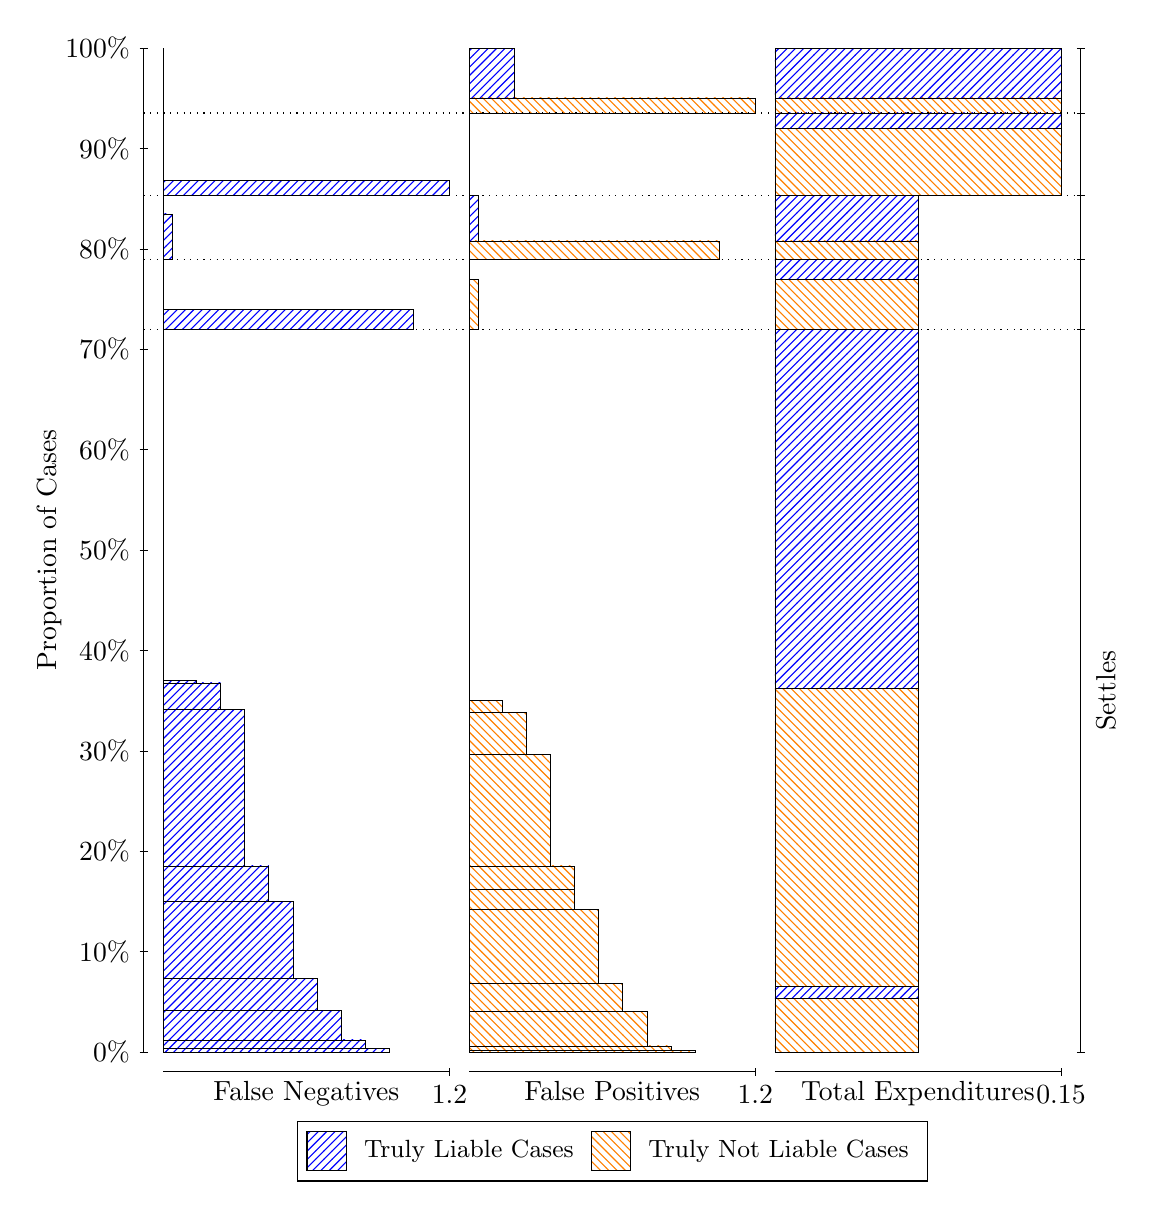
\begin{tikzpicture}
\draw[black, very thin] (1.5,1.75) -- (1.5,14.5);
\node[rotate=90, anchor=center] at (0.3, 8.125) {Proportion of Cases};
\draw[black, very thin] (1.45,1.75) -- (1.55,1.75);
\node[anchor=east] at (1.45, 1.75) {0\%};
\draw[black, very thin] (1.45,3.025) -- (1.55,3.025);
\node[anchor=east] at (1.45, 3.025) {10\%};
\draw[black, very thin] (1.45,4.3) -- (1.55,4.3);
\node[anchor=east] at (1.45, 4.3) {20\%};
\draw[black, very thin] (1.45,5.575) -- (1.55,5.575);
\node[anchor=east] at (1.45, 5.575) {30\%};
\draw[black, very thin] (1.45,6.85) -- (1.55,6.85);
\node[anchor=east] at (1.45, 6.85) {40\%};
\draw[black, very thin] (1.45,8.125) -- (1.55,8.125);
\node[anchor=east] at (1.45, 8.125) {50\%};
\draw[black, very thin] (1.45,9.4) -- (1.55,9.4);
\node[anchor=east] at (1.45, 9.4) {60\%};
\draw[black, very thin] (1.45,10.675) -- (1.55,10.675);
\node[anchor=east] at (1.45, 10.675) {70\%};
\draw[black, very thin] (1.45,11.95) -- (1.55,11.95);
\node[anchor=east] at (1.45, 11.95) {80\%};
\draw[black, very thin] (1.45,13.225) -- (1.55,13.225);
\node[anchor=east] at (1.45, 13.225) {90\%};
\draw[black, very thin] (1.45,14.5) -- (1.55,14.5);
\node[anchor=east] at (1.45, 14.5) {100\%};

\draw[black, very thin] (13.4,1.75) -- (13.4,14.5);
\draw[black, very thin] (13.35,1.75) -- (13.45,1.75);
\node[anchor=west] at (13.35, 1.75) {};
\draw[black, very thin] (13.35,10.927) -- (13.45,10.927);
\node[anchor=west] at (13.35, 10.927) {};
\draw[black, very thin] (13.35,11.817) -- (13.45,11.817);
\node[anchor=west] at (13.35, 11.817) {};
\draw[black, very thin] (13.35,12.629) -- (13.45,12.629);
\node[anchor=west] at (13.35, 12.629) {};
\draw[black, very thin] (13.35,13.675) -- (13.45,13.675);
\node[anchor=west] at (13.35, 13.675) {};
\draw[black, very thin] (13.35,14.5) -- (13.45,14.5);
\node[anchor=west] at (13.35, 14.5) {};

\draw[black, very thin, pattern color=blue, pattern=north east lines] (1.75,1.75) rectangle (4.6184,1.7994);
\draw[black, very thin, pattern color=blue, pattern=north east lines] (1.75,1.7994) rectangle (4.3125,1.9047);
\draw[black, very thin, pattern color=blue, pattern=north east lines] (1.75,1.9047) rectangle (4.0065,2.2766);
\draw[black, very thin, pattern color=blue, pattern=north east lines] (1.75,2.2766) rectangle (3.7005,2.6839);
\draw[black, very thin, pattern color=blue, pattern=north east lines] (1.75,2.6839) rectangle (3.3946,3.6608);
\draw[black, very thin, pattern color=blue, pattern=north east lines] (1.75,3.6608) rectangle (3.0886,4.1122);
\draw[black, very thin, pattern color=blue, pattern=north east lines] (1.75,4.1122) rectangle (2.7826,6.1057);
\draw[black, very thin, pattern color=blue, pattern=north east lines] (1.75,6.1057) rectangle (2.4767,6.4371);
\draw[black, very thin, pattern color=blue, pattern=north east lines] (1.75,6.4371) rectangle (2.1707,6.4644);
\draw[black, very thin, pattern color=orange, pattern=north west lines] (1.75,6.4644) rectangle (1.75,10.927);
\draw[black, very thin, pattern color=blue, pattern=north east lines] (1.75,10.927) rectangle (4.9244,11.183);
\draw[black, very thin, pattern color=orange, pattern=north west lines] (1.75,11.183) rectangle (1.75,11.817);
\draw[black, very thin, pattern color=blue, pattern=north east lines] (1.75,11.817) rectangle (1.8647,12.395);
\draw[black, very thin, pattern color=orange, pattern=north west lines] (1.75,12.395) rectangle (1.75,12.629);
\draw[black, very thin, pattern color=blue, pattern=north east lines] (1.75,12.629) rectangle (5.3833,12.822);
\draw[black, very thin, pattern color=orange, pattern=north west lines] (1.75,12.822) rectangle (1.75,13.675);
\draw[black, very thin, pattern color=orange, pattern=north west lines] (1.75,13.675) rectangle (1.75,13.868);
\draw[black, very thin, pattern color=blue, pattern=north east lines] (1.75,13.868) rectangle (1.75,14.5);
\draw[black, very thin, pattern color=orange, pattern=north west lines] (5.6333,1.75) rectangle (8.5018,1.7664);
\draw[black, very thin, pattern color=orange, pattern=north west lines] (5.6333,1.7664) rectangle (8.1958,1.826);
\draw[black, very thin, pattern color=orange, pattern=north west lines] (5.6333,1.826) rectangle (7.8898,2.2687);
\draw[black, very thin, pattern color=orange, pattern=north west lines] (5.6333,2.2687) rectangle (7.5839,2.6215);
\draw[black, very thin, pattern color=orange, pattern=north west lines] (5.6333,2.6215) rectangle (7.2779,3.5606);
\draw[black, very thin, pattern color=orange, pattern=north west lines] (5.6333,3.5606) rectangle (6.9719,3.8167);
\draw[black, very thin, pattern color=orange, pattern=north west lines] (5.6333,3.8167) rectangle (6.9719,4.1145);
\draw[black, very thin, pattern color=orange, pattern=north west lines] (5.6333,4.1145) rectangle (6.666,5.5327);
\draw[black, very thin, pattern color=orange, pattern=north west lines] (5.6333,5.5327) rectangle (6.36,6.0602);
\draw[black, very thin, pattern color=orange, pattern=north west lines] (5.6333,6.0602) rectangle (6.054,6.2126);
\draw[black, very thin, pattern color=blue, pattern=north east lines] (5.6333,6.2126) rectangle (5.6333,10.927);
\draw[black, very thin, pattern color=orange, pattern=north west lines] (5.6333,10.927) rectangle (5.7481,11.56);
\draw[black, very thin, pattern color=blue, pattern=north east lines] (5.6333,11.56) rectangle (5.6333,11.817);
\draw[black, very thin, pattern color=orange, pattern=north west lines] (5.6333,11.817) rectangle (8.8077,12.05);
\draw[black, very thin, pattern color=blue, pattern=north east lines] (5.6333,12.05) rectangle (5.7481,12.629);
\draw[black, very thin, pattern color=orange, pattern=north west lines] (5.6333,12.629) rectangle (5.6333,13.482);
\draw[black, very thin, pattern color=blue, pattern=north east lines] (5.6333,13.482) rectangle (5.6333,13.675);
\draw[black, very thin, pattern color=orange, pattern=north west lines] (5.6333,13.675) rectangle (9.2667,13.868);
\draw[black, very thin, pattern color=blue, pattern=north east lines] (5.6333,13.868) rectangle (6.207,14.5);
\draw[black, very thin, pattern color=orange, pattern=north west lines] (9.5167,1.75) rectangle (11.333,2.4299);
\draw[black, very thin, pattern color=blue, pattern=north east lines] (9.5167,2.4299) rectangle (11.333,2.5847);
\draw[black, very thin, pattern color=orange, pattern=north west lines] (9.5167,2.5847) rectangle (11.333,6.3674);
\draw[black, very thin, pattern color=blue, pattern=north east lines] (9.5167,6.3674) rectangle (11.333,10.927);
\draw[black, very thin, pattern color=orange, pattern=north west lines] (9.5167,10.927) rectangle (11.333,11.56);
\draw[black, very thin, pattern color=blue, pattern=north east lines] (9.5167,11.56) rectangle (11.333,11.817);
\draw[black, very thin, pattern color=orange, pattern=north west lines] (9.5167,11.817) rectangle (11.333,12.05);
\draw[black, very thin, pattern color=blue, pattern=north east lines] (9.5167,12.05) rectangle (11.333,12.629);
\draw[black, very thin, pattern color=orange, pattern=north west lines] (9.5167,12.629) rectangle (13.15,13.482);
\draw[black, very thin, pattern color=blue, pattern=north east lines] (9.5167,13.482) rectangle (13.15,13.675);
\draw[black, very thin, pattern color=orange, pattern=north west lines] (9.5167,13.675) rectangle (13.15,13.868);
\draw[black, very thin, pattern color=blue, pattern=north east lines] (9.5167,13.868) rectangle (13.15,14.5);
\draw[black, dotted] (1.5,10.927) -- (13.4,10.927);
\draw[black, dotted] (1.5,11.817) -- (13.4,11.817);
\draw[black, dotted] (1.5,12.629) -- (13.4,12.629);
\draw[black, dotted] (1.5,13.675) -- (13.4,13.675);
\draw[black, very thin] (1.75,1.5) -- (5.3833,1.5);
\node[anchor=north] at (3.5667, 1.5) {False Negatives};
\draw[black, very thin] (5.3833,1.45) -- (5.3833,1.55);
\node[anchor=north] at (5.3833, 1.45) {1.2};

\draw[black, very thin] (5.6333,1.5) -- (9.2667,1.5);
\node[anchor=north] at (7.45, 1.5) {False Positives};
\draw[black, very thin] (9.2667,1.45) -- (9.2667,1.55);
\node[anchor=north] at (9.2667, 1.45) {1.2};

\draw[black, very thin] (9.5167,1.5) -- (13.15,1.5);
\node[anchor=north] at (11.333, 1.5) {Total Expenditures};
\draw[black, very thin] (13.15,1.45) -- (13.15,1.55);
\node[anchor=north] at (13.15, 1.45) {0.15};

\node[black, centered, rotate=90] at (13.72, 6.3385) {Settles};





\draw (7.449999999999999,1.5) node[draw=none] (baseCoordinate) {};
\begin{scope}[align=center]
        \matrix[scale=0.5, draw=black, below=0.5cm of baseCoordinate, nodes={draw}, column sep=0.1cm]{
            \node[rectangle, draw, minimum width=0.5cm, minimum height=0.5cm, pattern=north east lines, pattern color=blue] {}; &
            \node[draw=none, font=\small] (B) {Truly Liable Cases}; &
            \node[rectangle, draw, minimum width=0.5cm, minimum height=0.5cm, pattern=north west lines, pattern color=orange] {}; &
            \node[draw=none, font=\small] (B) {Truly Not Liable Cases}; \\
            };
\end{scope}

\end{tikzpicture}
\end{document}